% This file was generated with po4a. Translate the source file.
%
\pdfobjcompresslevel=1 \documentclass[notes=hide]{beamer}
\usetheme[titlepagelogo=img2/cover]{LDN}

\usepackage[utf8]{inputenc}
\usepackage[francais]{babel}
\usepackage[T1]{fontenc}
\usepackage{tabularx, verbatim, xcolor, textpos}
\usepackage{lmodern, alltt, graphicx, ragged2e}
\usepackage{marvosym, multicol, textcomp, eurosym}

\definecolor{darkgreen}{RGB}{0,99,0}
\newcommand{\good}{{\color{green}\Smiley}}
\newcommand{\bad}{{\color{red}\Frowny}}
\colorlet{titre}{white} \setbeamercolor{normal text}{fg=white,bg=white}

\date{\textbf{AG FFDN 2015}}

\title{Internet³}
\subtitle{\vspace{10pt}\emph{Neutral Internet \& Home-hosted}}
\author{Neutrinet \\ Lorraine Data Network \\ YunoHost}
\begin{document}

\begin{frame}[t,plain]
\titlepage
  \begin{textblock}{}(10,-7)
    
\includegraphics[height=1.5cm]{img2/logo-ynh-black.pdf}
  \end{textblock}
  \begin{textblock}{}(9.5,-4)
    \includegraphics[height=1.2cm]{img2/logoldn}
  \end{textblock}
  \begin{textblock}{}(10,-1.5)
    
\includegraphics[height=1.5cm]{img2/logo-neutrinet}
  \end{textblock}\color{black}\textbf{OuiShareLabs May 2015}
\end{frame}

\watermarkon \watermarkoff

\setbeamercolor{background canvas}{bg=black}
\begin{frame}[t,plain]
\begin{center}
  \vspace{\fill}
    \includegraphics[width=230pt]{img2/logoldn}
  \vspace{\fill}
  \color{white}{\fontsize{30}{30}\selectfont Lorraine Data Network}
\end{center}
\end{frame}

\begin{frame}[t,plain]
  \begin{center}
    \vspace{\fill}
      \color{white}{\fontsize{60}{60}\selectfont libre, neutre}
    \vspace{\fill}
  \end{center}
\end{frame}

\begin{frame}[t,plain]
  \begin{center}
    \vspace{\fill}
      \color{white}{\fontsize{60}{60}\selectfont et décentralisé}
    \vspace{\fill}
  \end{center}
\end{frame}

\begin{frame}[t,plain]
  \begin{center}
    \vspace{\fill}
      \color{white}{\fontsize{40}{40}\selectfont Libre et neutre~?}
    \vspace{\fill}
  \end{center}
\end{frame}

\begin{frame}[t]
\frametitle{\textcolor{titre}{Whithout Internet³}}
  \color{red!60} \begin{center}
    \includegraphics[width=0.9\textwidth]{img2/connexion1.png}
  \end{center}
\end{frame}

\begin{frame}[t]
\frametitle{\textcolor{titre}{Whithout Internet³}}
  \begin{center}
    \includegraphics[width=0.9\textwidth]{img2/connexion2.png}
  \end{center}
\end{frame}

\begin{frame}[t]
\frametitle{\textcolor{titre}{Whithout Internet³}}
  \begin{center}
    \includegraphics[width=0.9\textwidth]{img2/connexion3.png}
  \end{center}
\end{frame}

\begin{frame}[t]
\frametitle{\textcolor{titre}{Whithout Internet³}}
  \begin{center}
    \includegraphics[width=0.9\textwidth]{img2/connexion4.png}
  \end{center}
\end{frame}

\begin{frame}[t]
\frametitle{\textcolor{titre}{Problems~?}}
  \begin{center}
    \includegraphics[width=0.9\textwidth]{img2/connexion5.png}
  \end{center}
\end{frame}

\begin{frame}
\frametitle{\textcolor{titre}{Problems}}
  \begin{itemize}
    \item Traffic shaping (Comcast Vs Netflix) \pause
    \item Port blocking (port 25) \pause
    \item Dynamic IP addressing / no IPv6 \pause
    \item Censorship (DNS hijacking) \pause
    \item Surveillance \pause
    \item Use personal data
  \end{itemize}
\end{frame}

\begin{frame}[t]
		  \frametitle{\textcolor{titre}{Promesse de ne pas respecter ma vie privée}}
\begin{center}
\vfill
\includegraphics[width=.75\textwidth]{img2/03g-cgu.png}
\vfill
\end{center}
\end{frame}

\begin{frame}[t]
\frametitle{\textcolor{titre}{Whith Internet³}}
		  \color{red!60} \begin{center}
		  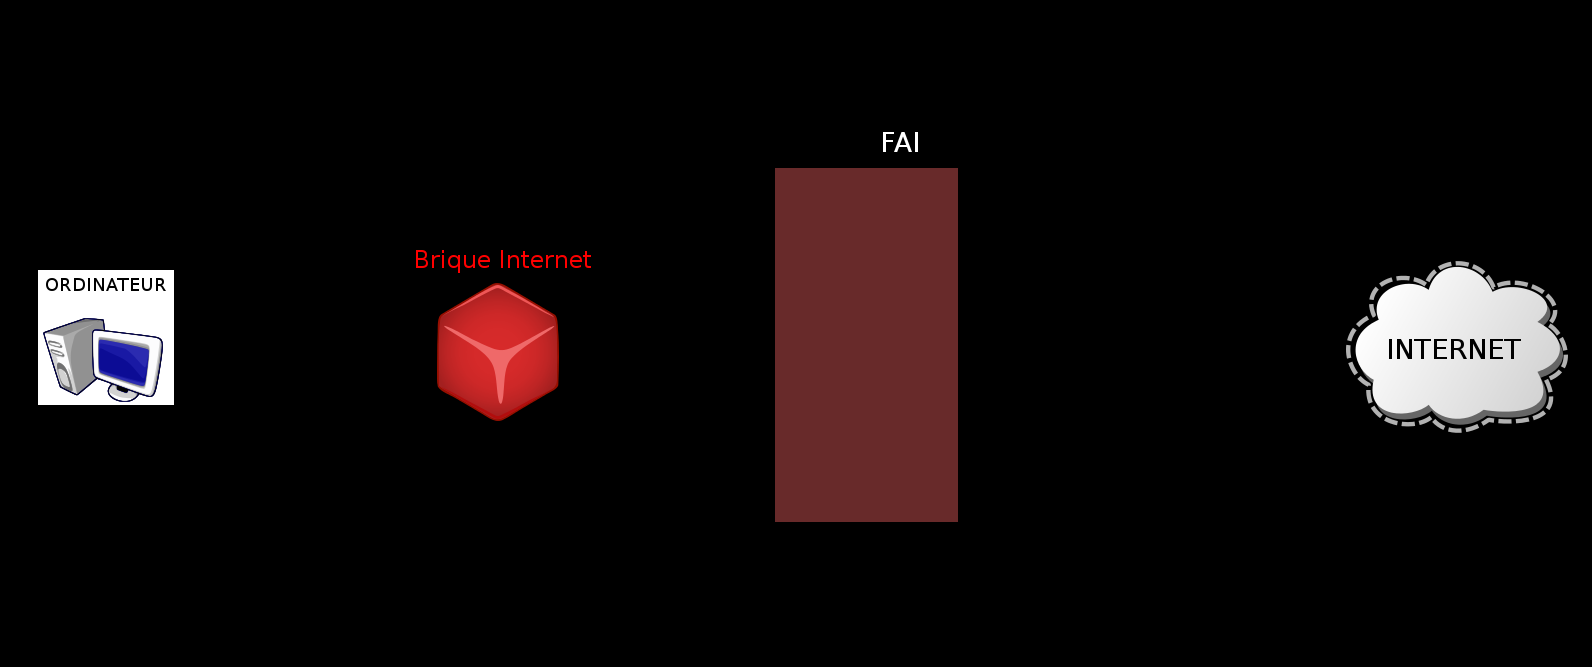
\includegraphics[width=0.9\textwidth]{img2/connexion11.png}
		  \end{center}
\end{frame}
\begin{frame}[t]
\frametitle{\textcolor{titre}{Whith Internet³}}
		  \begin{center}
		  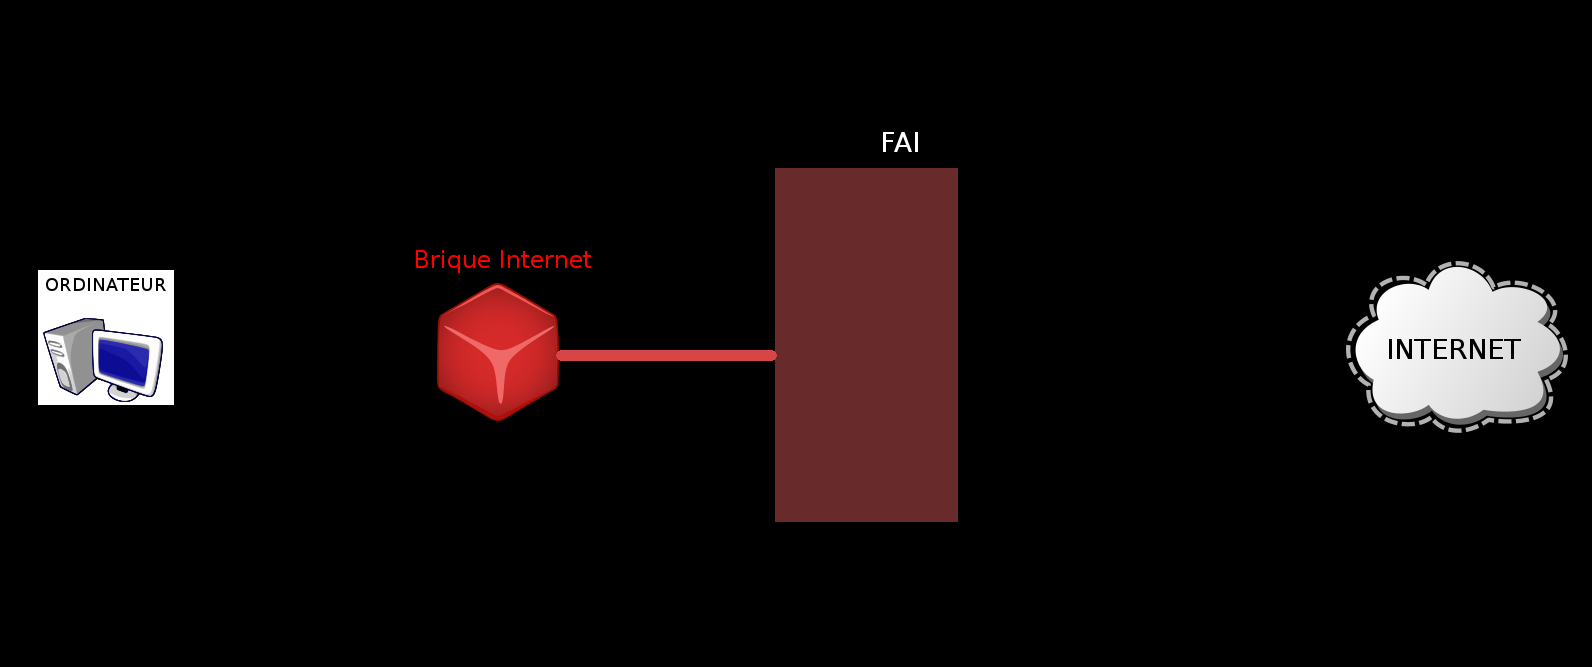
\includegraphics[width=0.9\textwidth]{img2/connexion12.png}
		  \end{center}
\end{frame}
\begin{frame}[t]
\frametitle{\textcolor{titre}{Whith Internet³}}
		  \begin{center}
		  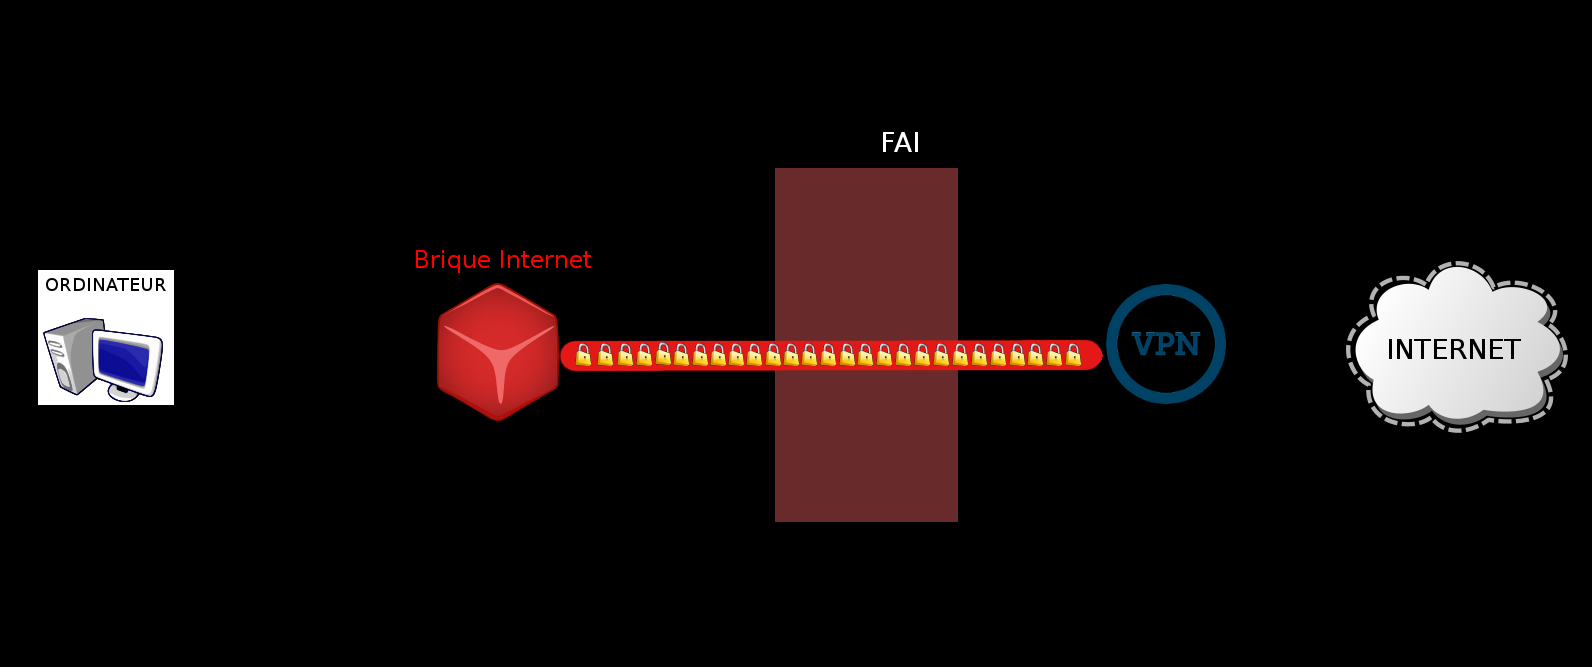
\includegraphics[width=0.9\textwidth]{img2/connexion13.png}
		  \end{center}
\end{frame}
\begin{frame}[t]
\frametitle{\textcolor{titre}{Whith Internet³}}
		  \begin{center}
		  \includegraphics[width=0.9\textwidth]{img2/connexion14.png}
		  \end{center}
\end{frame}

\begin{frame}[t]
		  \frametitle{\textcolor{titre}{Whith Internet³}}
		  \begin{center}
		  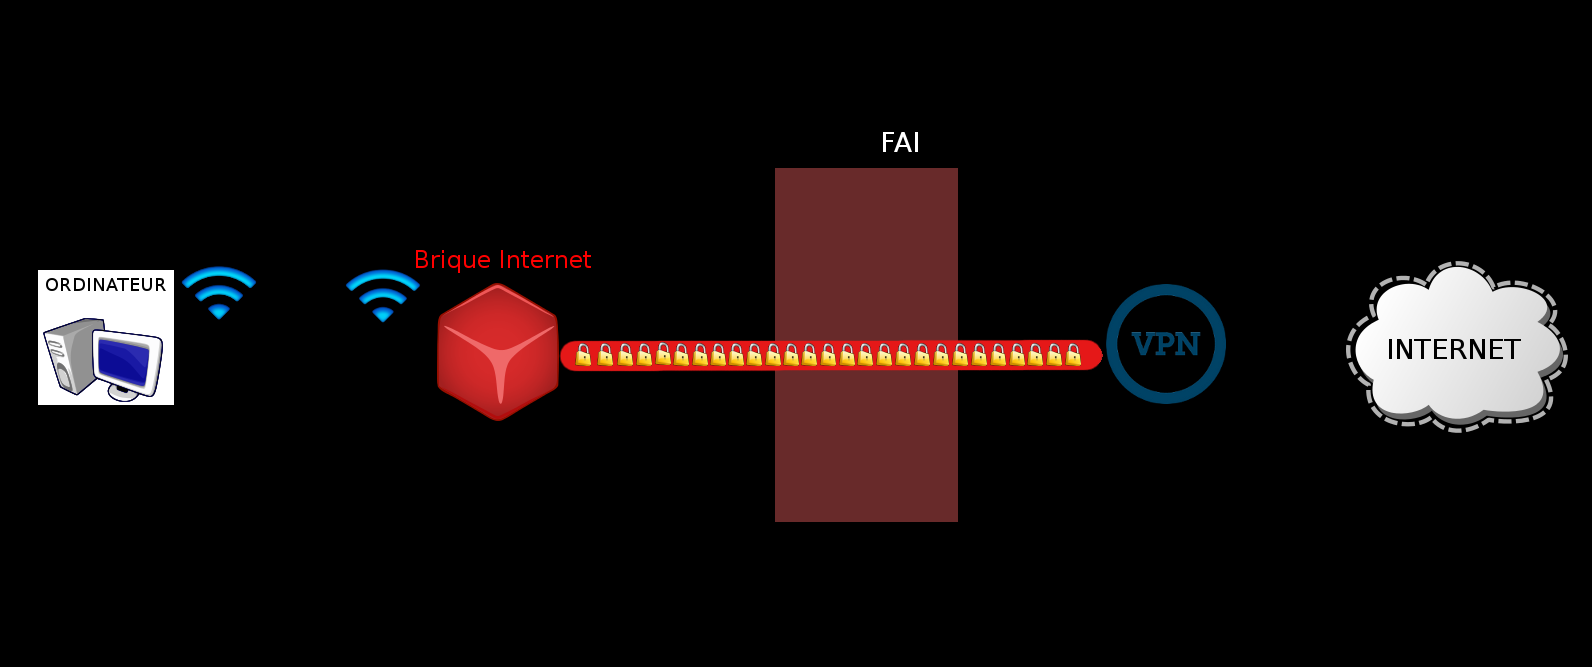
\includegraphics[width=0.9\textwidth]{img2/connexion15.png}
		  \end{center}
\end{frame}


\begin{frame}[t]
		  \frametitle{\textcolor{titre}{Whith Internet³}}
		  \begin{center}
		  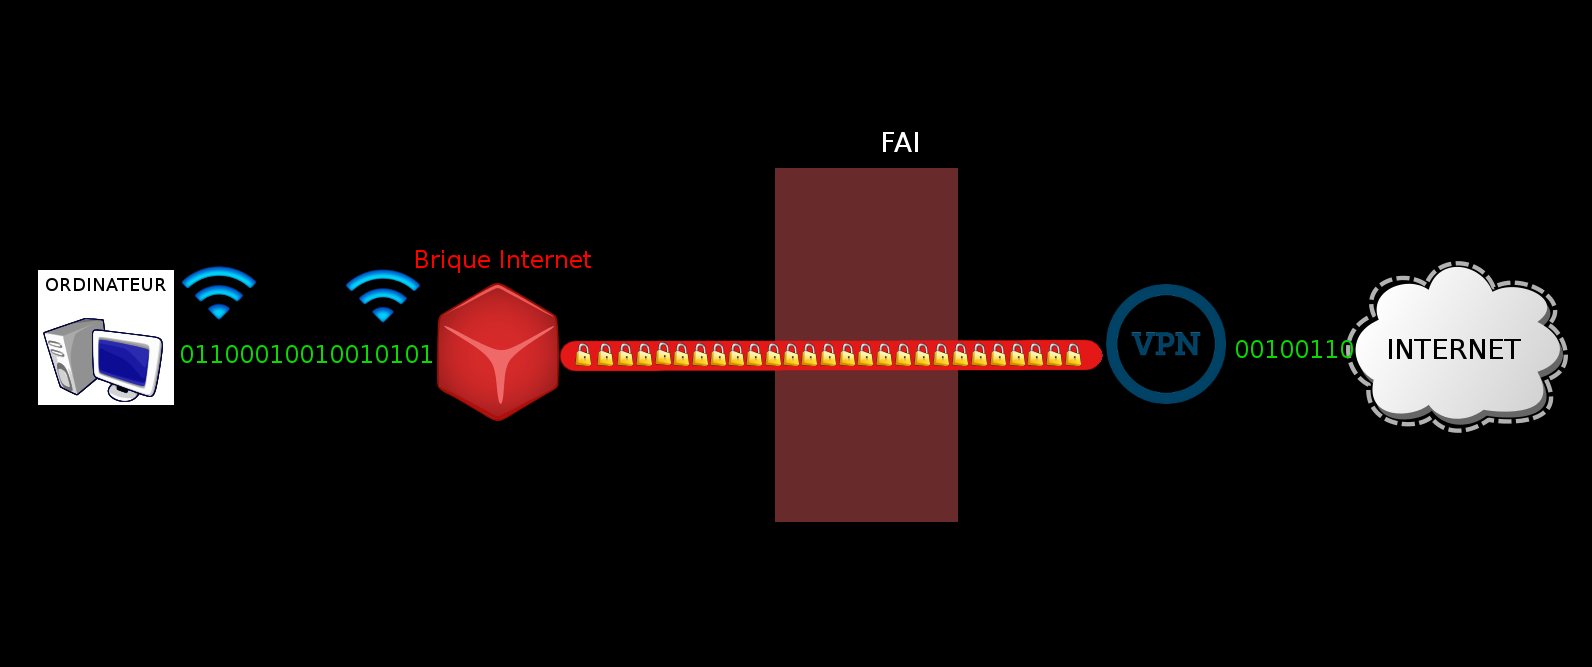
\includegraphics[width=0.9\textwidth]{img2/connexion16.png}
		  \end{center}
\end{frame}

\begin{frame}
		  \frametitle{\textcolor{titre}{Problems~?}}
					 \begin{itemize}
								\item Traffic shaping (Comcast Vs Netflix)
								\item Port blocking (port 25)
								\item Dynamic IP addressing
								\item Censorship (DNS hijacking)
								\item Surveillance
								\item Use personal data
					\end{itemize}
\end{frame}

\begin{frame}
		  \frametitle{\textcolor{titre}{Problems~?}}
					 \begin{itemize}
								\item
								\item Port blocking (port 25)
								\item Dynamic IP addressing
								\item Censorship (DNS hijacking)
								\item Surveillance
								\item Use personal data
					\end{itemize}
\end{frame}

\begin{frame}
		  \frametitle{\textcolor{titre}{Problems~?}}
					 \begin{itemize}
								\item
								\item
								\item Dynamic IP addressing
								\item Censorship (DNS hijacking)
								\item Surveillance
								\item Use personal data
					\end{itemize}
\end{frame}





\begin{frame}
		  \frametitle{\textcolor{titre}{Problems~?}}
					 \begin{itemize}
								\item
								\item
								\item
								\item Censorship (DNS hijacking)
								\item Surveillance
								\item Use personal data
					\end{itemize}
\end{frame}

\begin{frame}
		  \frametitle{\textcolor{titre}{Problems~?}}
					 \begin{itemize}
								\item
								\item
								\item
								\item
								\item Surveillance
								\item Use personal data
					\end{itemize}
\end{frame}

\begin{frame}
		  \frametitle{\textcolor{titre}{Problems~?}}
					 \begin{itemize}
								\item
								\item
								\item
								\item
								\item
								\item Use personal data
					\end{itemize}
\end{frame}

\begin{frame}[t,plain]
\begin{center}
\vspace{\fill}
	   \color{white}{\fontsize{60}{60}\selectfont libre, neutre!}
	   \vspace{\fill}
\end{center}
\end{frame}

\begin{frame}[t,plain]
\begin{center}
\vspace{\fill}
	   \color{white}{\fontsize{60}{60}\selectfont Décentralisé ?}
	   \vspace{\fill}
\end{center}
\end{frame}
\begin{frame}[t]
		  \frametitle{\textcolor{titre}{Comment communique-t-on sur Internet ?}}
\begin{center}
\vfill
\includegraphics[width=.7\textwidth]{img2/15a-capture-gmailfbskype.png}
\vfill
\end{center}
\end{frame}

\begin{frame}[t]
		  \frametitle{\textcolor{titre}{What do you agree when you use Google's
services~?}}
		  \vspace{4mm}
	   \begin{justify}
		   "\emph{When you upload, submit, store, send or receive content to or through
host, store, \textbf{reproduce, modify, create derivative works} [..]
communicate, publish, publicly perform, publicly display and distribute such
content))}"
			   \end{justify}
\end{frame}

\begin{frame}[t]
		  \frametitle{\textcolor{titre}{Ce que vous acceptez chez Facebook}}
		  \vspace{4mm}
\begin{justify}
						   « \emph{Pour le contenu protégé par les droits de propriété intellectuelle,
comme les photos ou vidéos, [...] \textbf{vous nous accordez une licence}
non-exclusive, \textbf{transférable, sous-licenciable}, sans redevance et
mondiale \textbf{pour l'utilisation des contenus de propriété intellectuelle
que vous publiez} sur Facebook ou en relation à Facebook} »
							   \end{justify}
								\end{frame}

\begin{frame}[t]
\frametitle{\textcolor{titre}{Pendant combien de temps chez Google~?}}
   \vspace{4mm}
		  \begin{justify}
		  « \emph{Cette autorisation demeure pour toute la durée légale de protection
de votre contenu, \textbf{même si vous cessez d’utiliser nos Services}.} »
		  \end{justify}
	   \vspace{4mm}
\end{frame}

\begin{frame}[t]
\frametitle{\textcolor{titre}{Pendant combien de temps chez Facebook}}
		  \vfill
\begin{justify}
	   « \emph{Cette licence de propriété intellectuelle \textbf{se termine lorsque
vous supprimez vos contenus} de propriété intellectuelle ou votre compte,
\textbf{sauf si votre compte est partagé avec d'autres personnes} qui ne
l'ont pas supprimé.} »\\
\end{justify}
\vfill
\begin{justify}
		   « \emph{Lorsque vous supprimez votre contenu [...], vous comprenez que
\textbf{les contenus supprimés peuvent persister dans des copies} de
sauvegarde pendant \textbf{un certain temps}.} »
\end{justify}
\end{frame}

\begin{frame}[t]
\frametitle{\textcolor{titre}{And with Internet³,cela se passe comment~?}}
\pause

\begin{center}

\includegraphics[width=\textwidth]{img2/yunohost_rien.png}
\end{center}
\end{frame}

\begin{frame}[t]
\begin{center}
\vfill
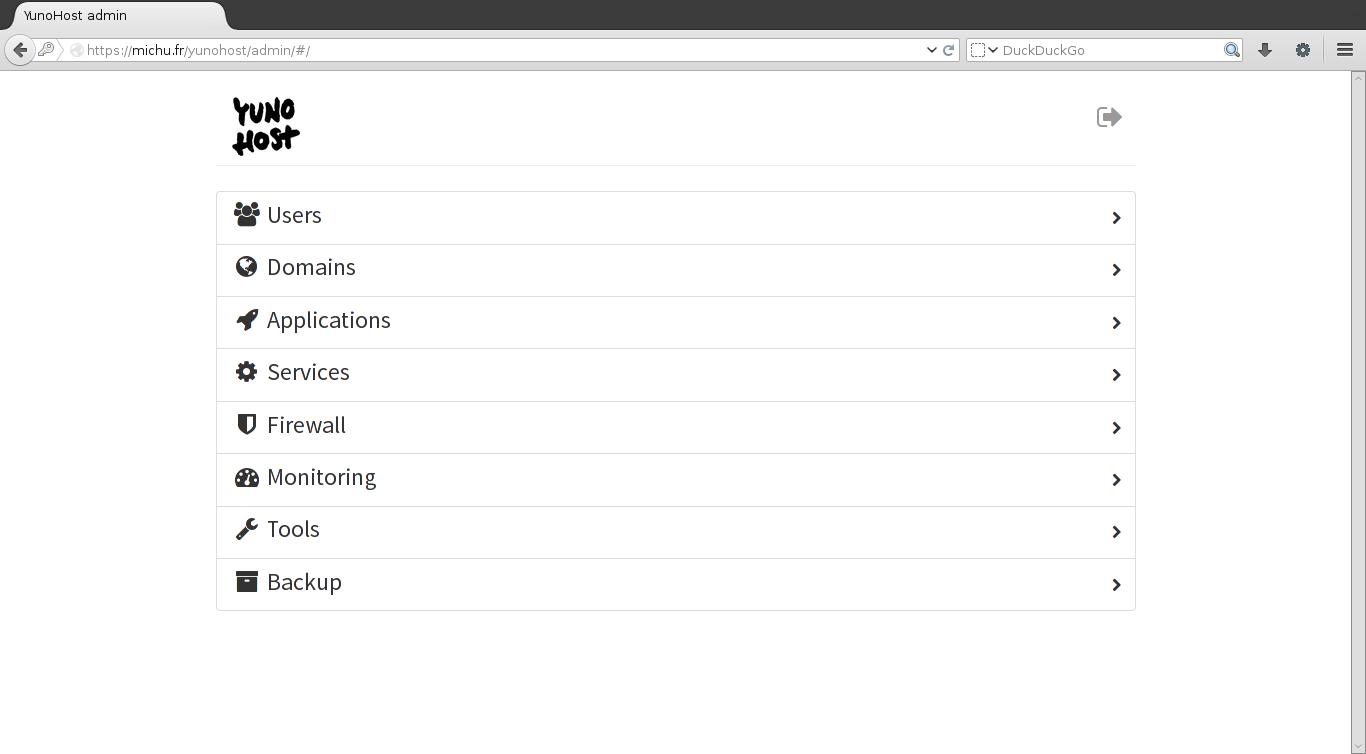
\includegraphics[width=\textwidth]{img2/17a-capture-yunohost.png}
\vfill
\end{center}
\end{frame}

\begin{frame}[t]
\begin{center}
\vfill
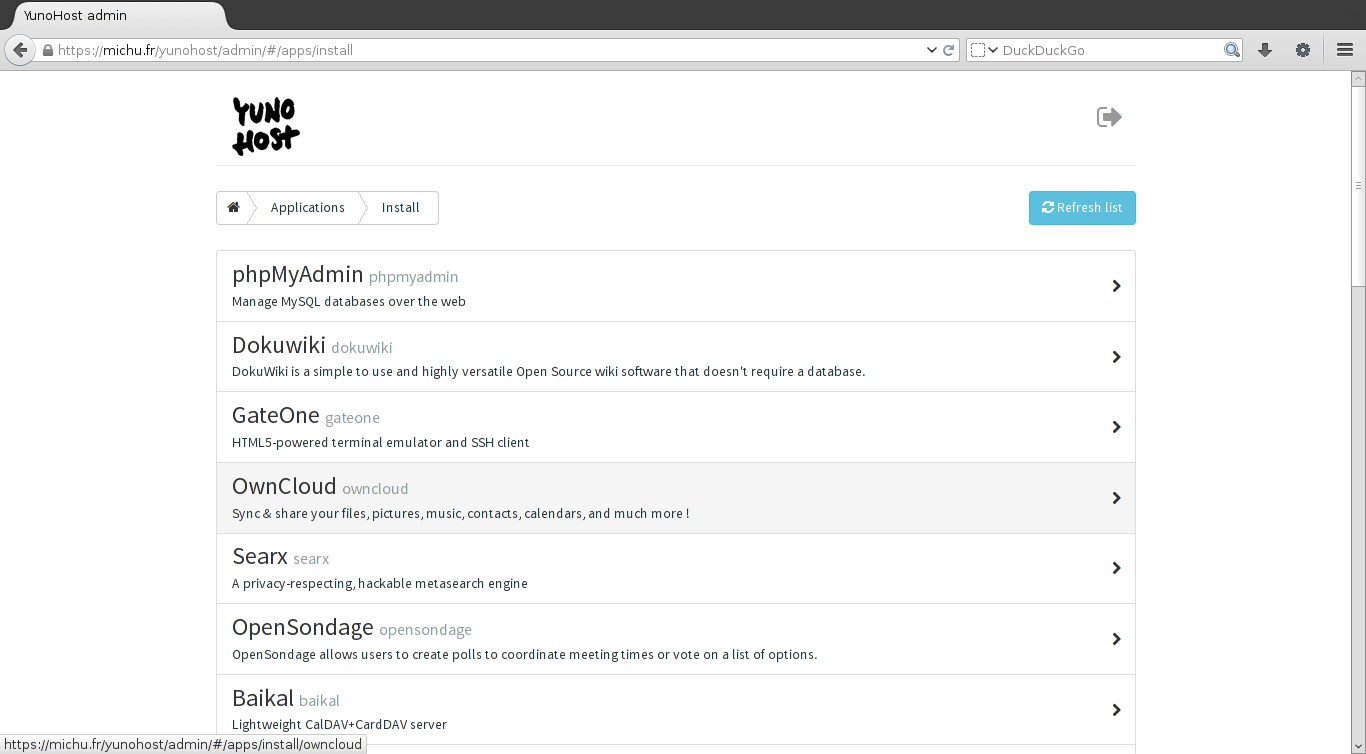
\includegraphics[width=\textwidth]{img2/19-capture-yunohostapps.png}
\vfill
\end{center}
\end{frame}

\begin{frame}[t,plain]
\begin{center}
\vspace{\fill}
	   \color{white}{\fontsize{60}{60}\selectfont Décentralisé !}
	   \vspace{\fill}
\end{center}
\end{frame}


\begin{frame}[t]
\frametitle{\textcolor{titre}{Combien ça coute…?}}
  \begin{center}
    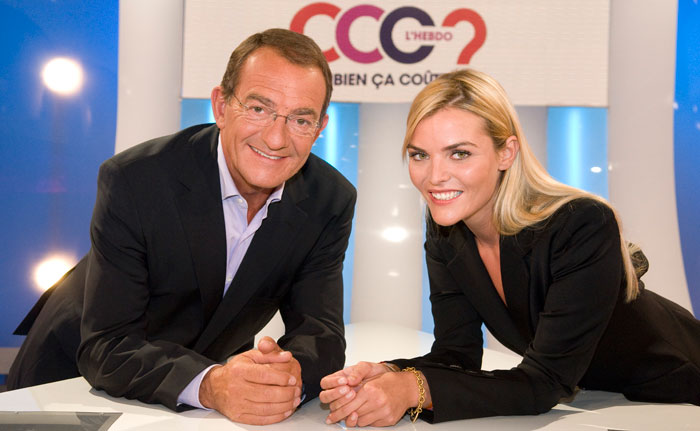
\includegraphics[width=0.9\textwidth]{img2/combiencacoute.jpg}
  \end{center}
\end{frame}

\begin{frame}[t]
\frametitle{\textcolor{titre}{Olimex board}}
  \begin{center}
    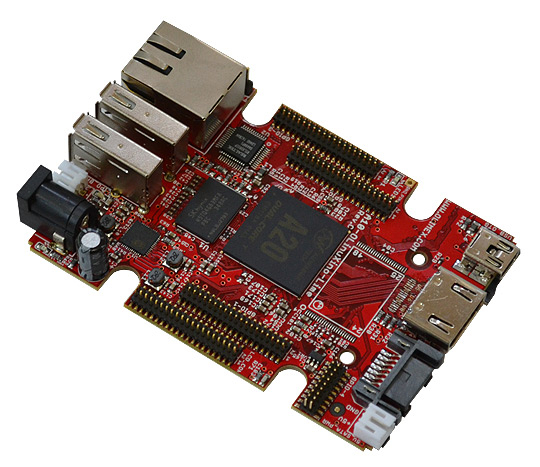
\includegraphics[width=0.7\textwidth]{img2/olimex.jpg}
  \end{center}
\end{frame}

\begin{frame}[t]
\frametitle{\textcolor{titre}{Box}}
  \begin{center}
    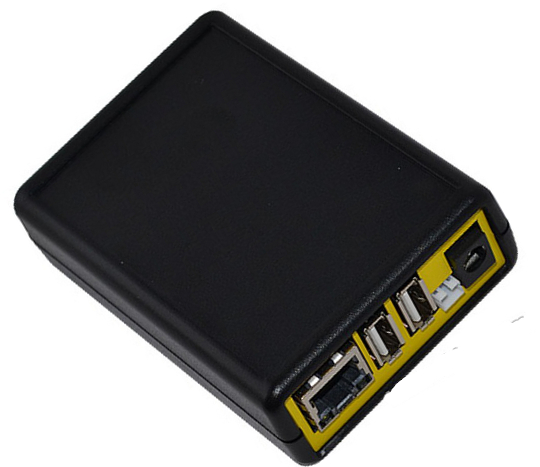
\includegraphics[width=0.7\textwidth]{img2/olimex-boite.jpg}
  \end{center}
\end{frame}
\begin{frame}[t]
\frametitle{\textcolor{titre}{Power supply}}
  \begin{center}
    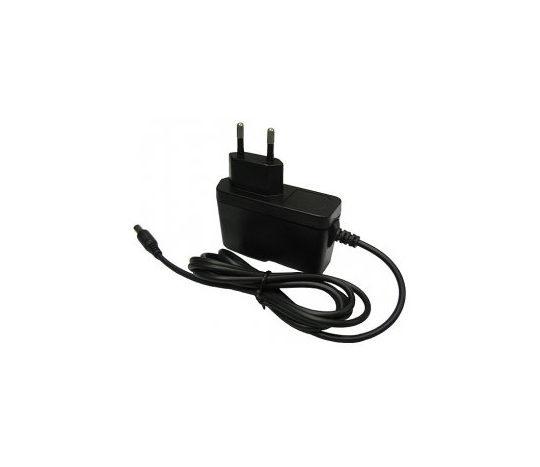
\includegraphics[width=0.7\textwidth]{img2/adaptateur.jpg}
  \end{center}
\end{frame}

\begin{frame}[t]
\frametitle{\textcolor{titre}{Wifi antenna}}
  \begin{center}
    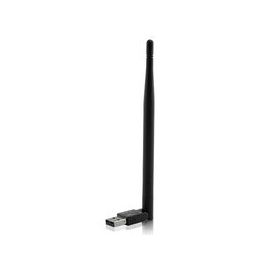
\includegraphics[width=0.6\textwidth]{img2/antenne.jpg}
  \end{center}
\end{frame}

\begin{frame}[t]
\frametitle{\textcolor{titre}{Memory card}}
  \begin{center}
    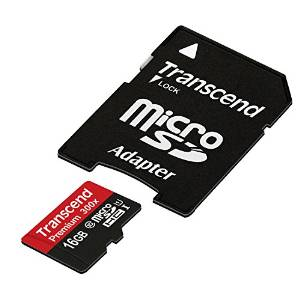
\includegraphics[width=0.6\textwidth]{img2/cartemem.jpg}
  \end{center}
\end{frame}

\begin{frame}[t]{}
\begin{center}
\vfill
\vfill{\Large Approximately \textbf{70\euro{} for 1 complete$^*$} Cube \\ (taxes
included)}
\vspace{1cm}

{\Large Environ \textbf{7 \euro{} / months} for a \\ \textbf{accès VPN}
associative}
\vspace{1cm}
\vfill

{\footnotesize \emph{* for a grouped order > 9 Cube, otherwise 80\euro}}
\vfill
\end{center}
\end{frame}

\begin{frame}[t]
\frametitle{\textcolor{titre}{I have a Cube !}}
\begin{center}
  \vfill
    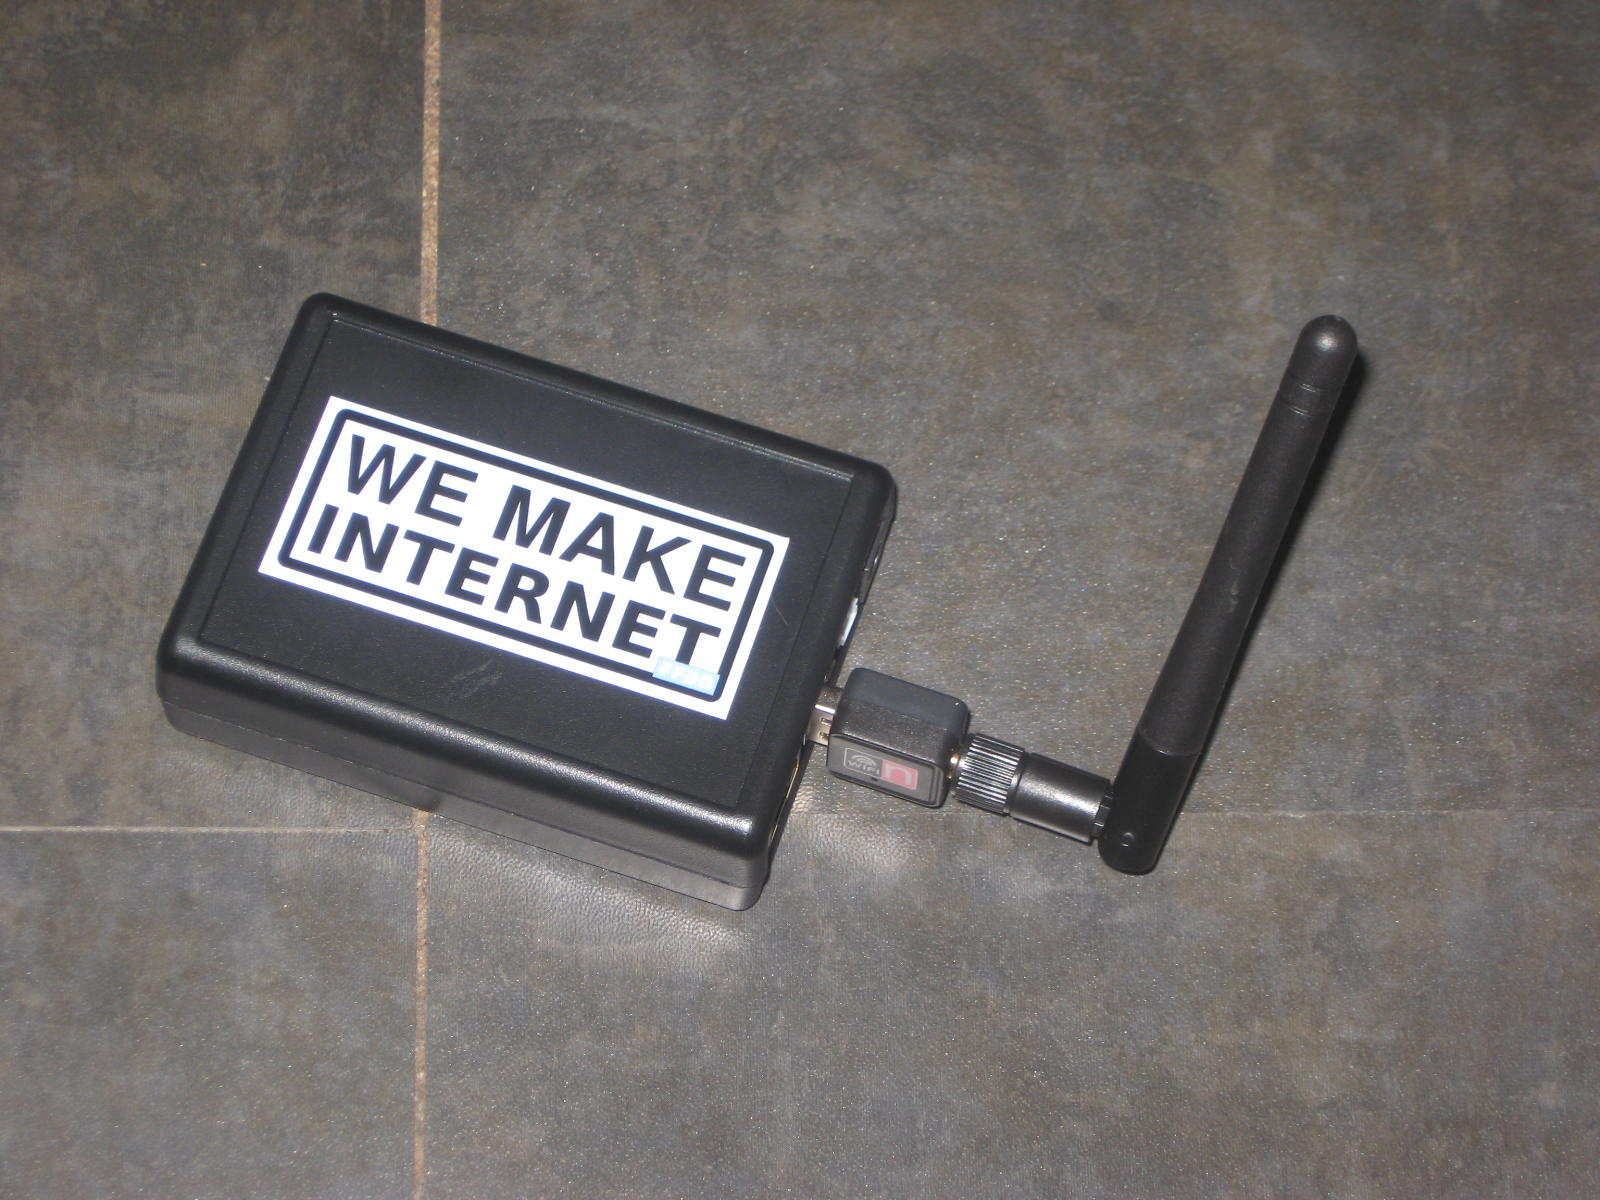
\includegraphics[width=.75\textwidth]{img2/04-photo-boitier.jpg}
  \vfill
\end{center}
\end{frame}

\begin{frame}[t]
\frametitle{\textcolor{titre}{I connecte my Cube to my ISP modem/router}}
\begin{center}
\vfill
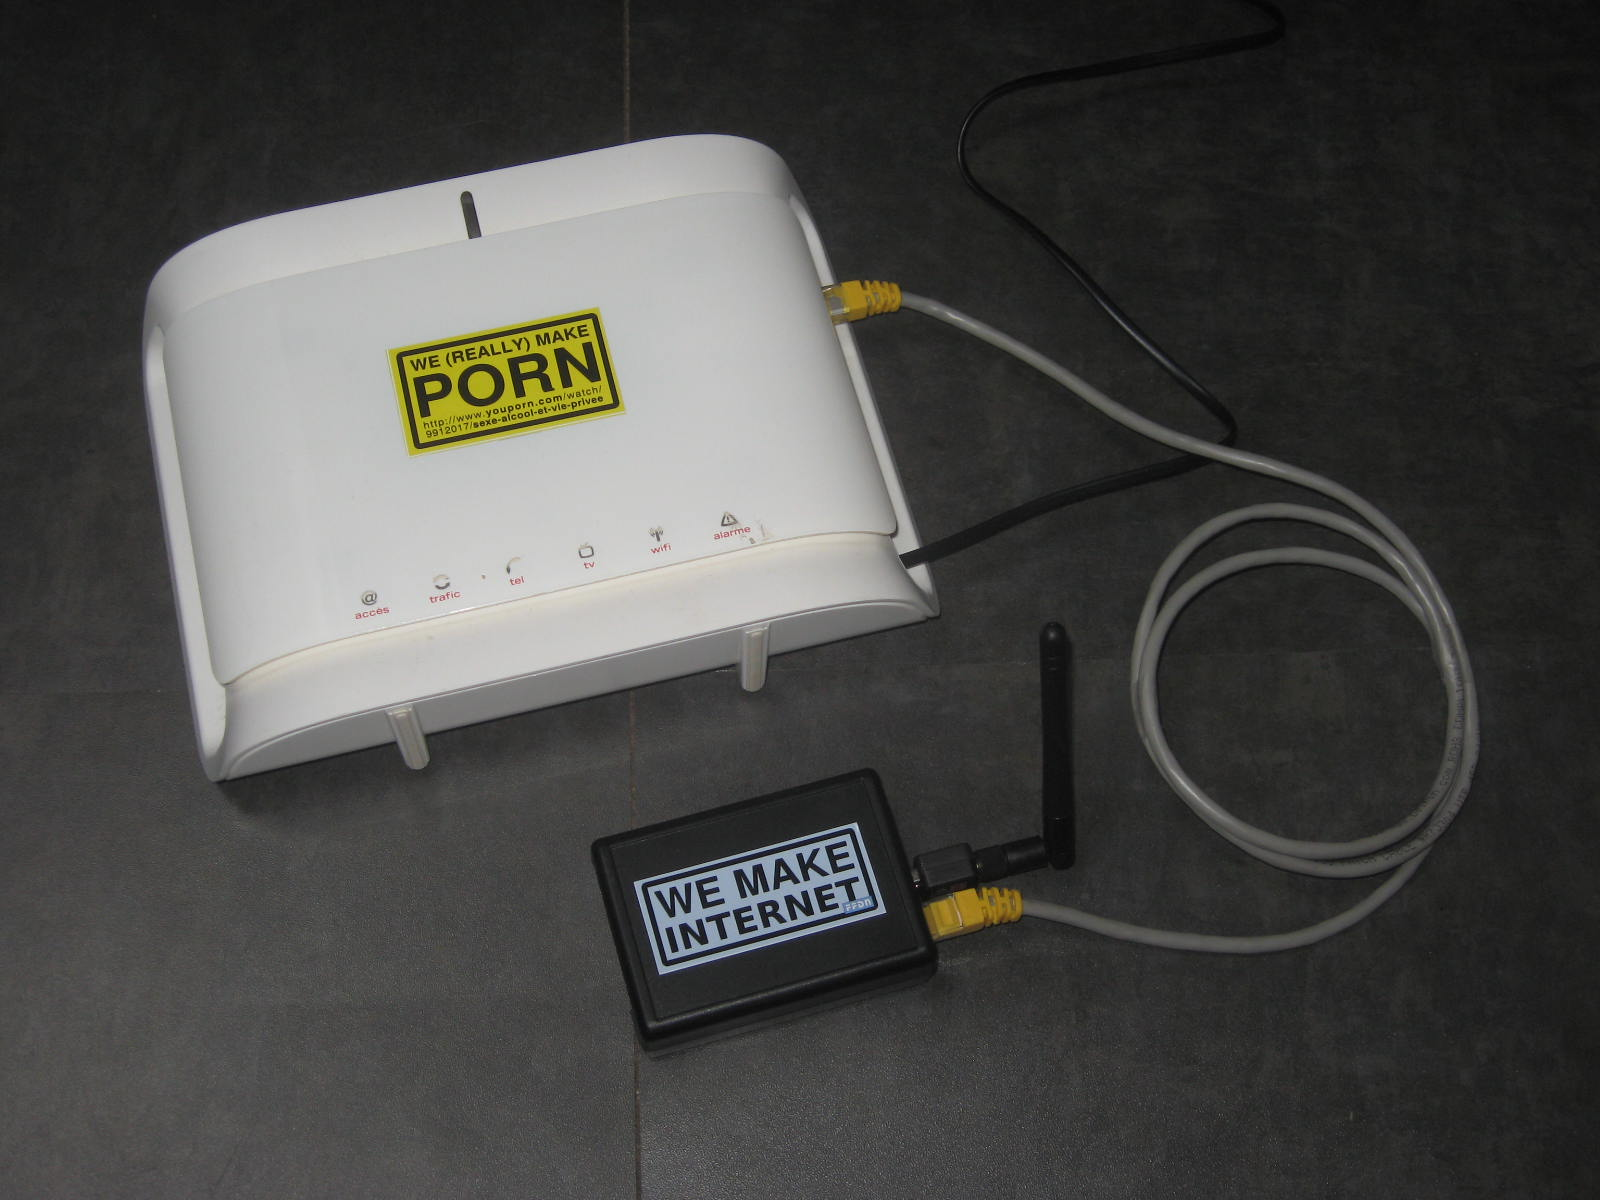
\includegraphics[width=.75\textwidth]{img2/05-photo-neufboxboitier.jpg}
\vfill
\end{center}
\end{frame}

\begin{frame}[t]
\frametitle{\textcolor{titre}{It does take no place}}
\begin{center}
\vfill
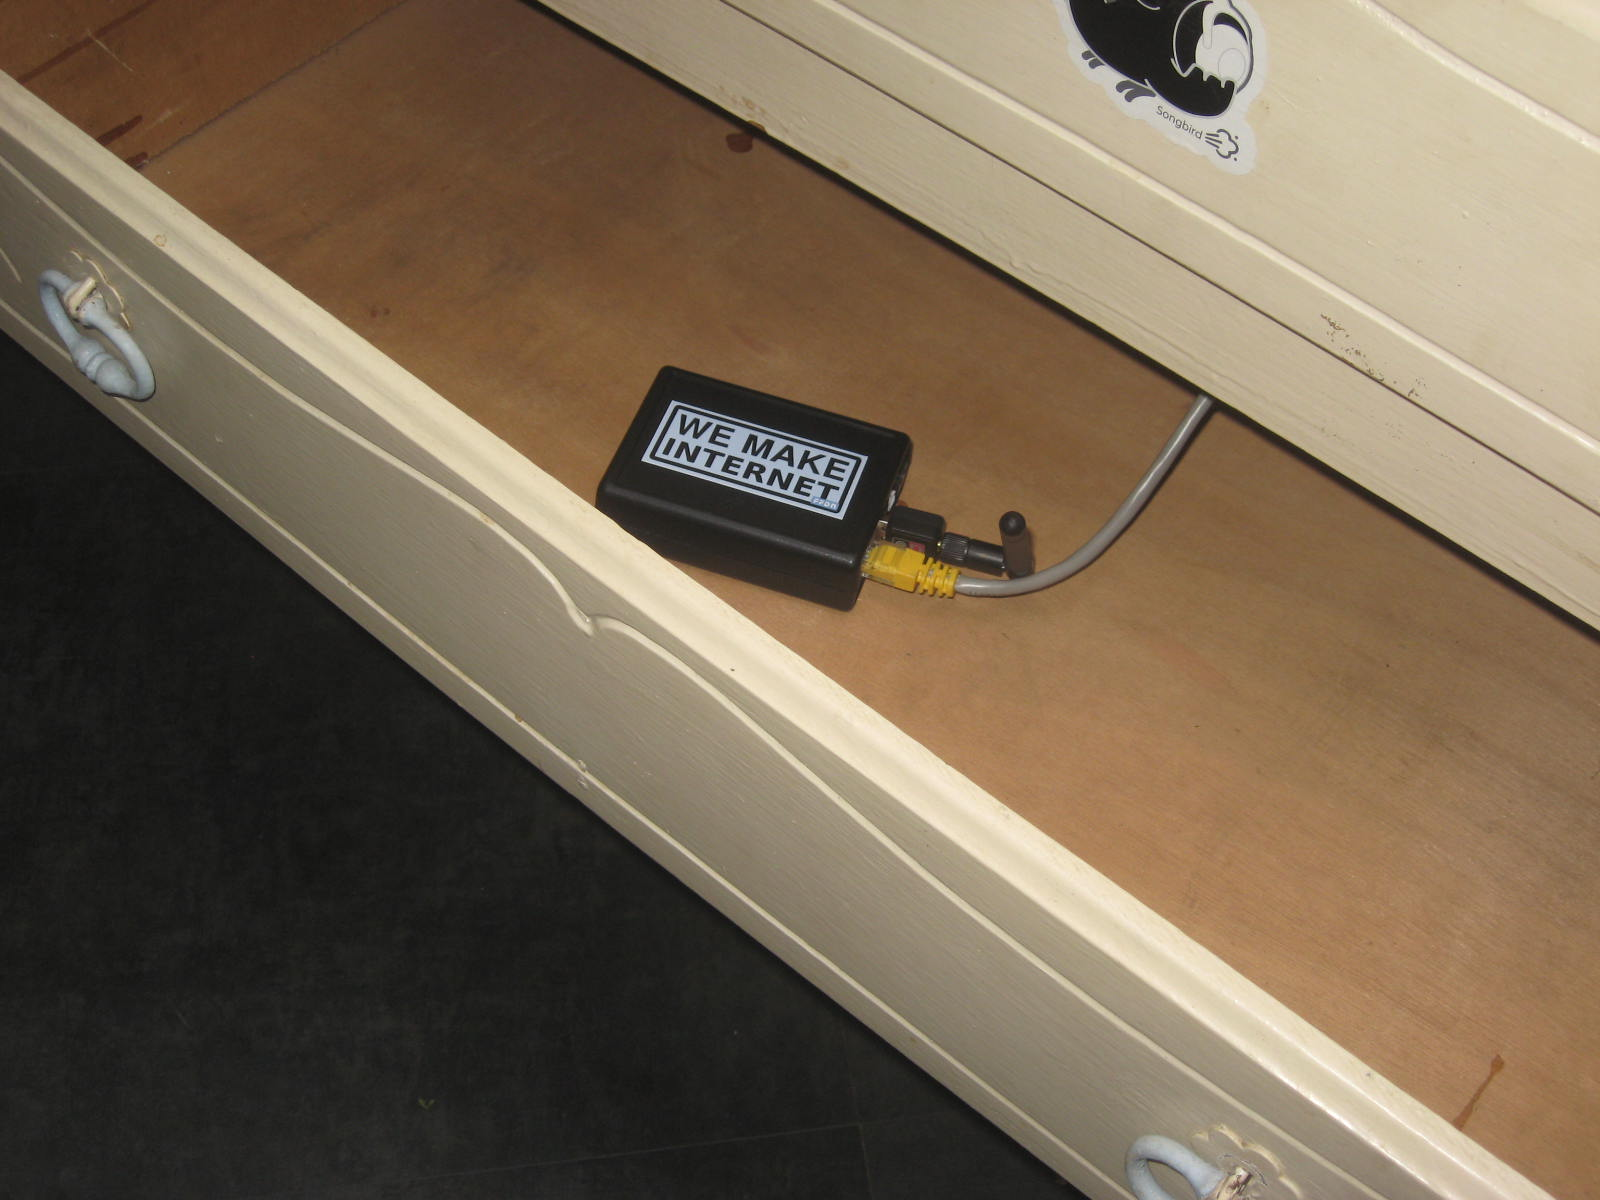
\includegraphics[width=.75\textwidth]{img2/16-photo-boitiercommode.jpg}
\vfill
\end{center}
\end{frame}

\begin{frame}[t]
\frametitle{\textcolor{titre}{And it's works out of the Cube}}
\begin{center}
\vfill
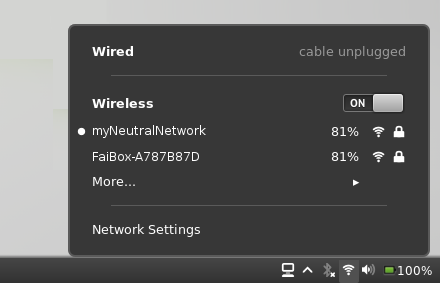
\includegraphics[width=.8\textwidth]{img2/06-capture-wifiboitier.png}
\vfill
\end{center}
\end{frame}

\begin{frame}[t]
\frametitle{\textcolor{titre}{I can still use other services of my ISP (like
phone, TV)}}
\begin{center}
\vfill
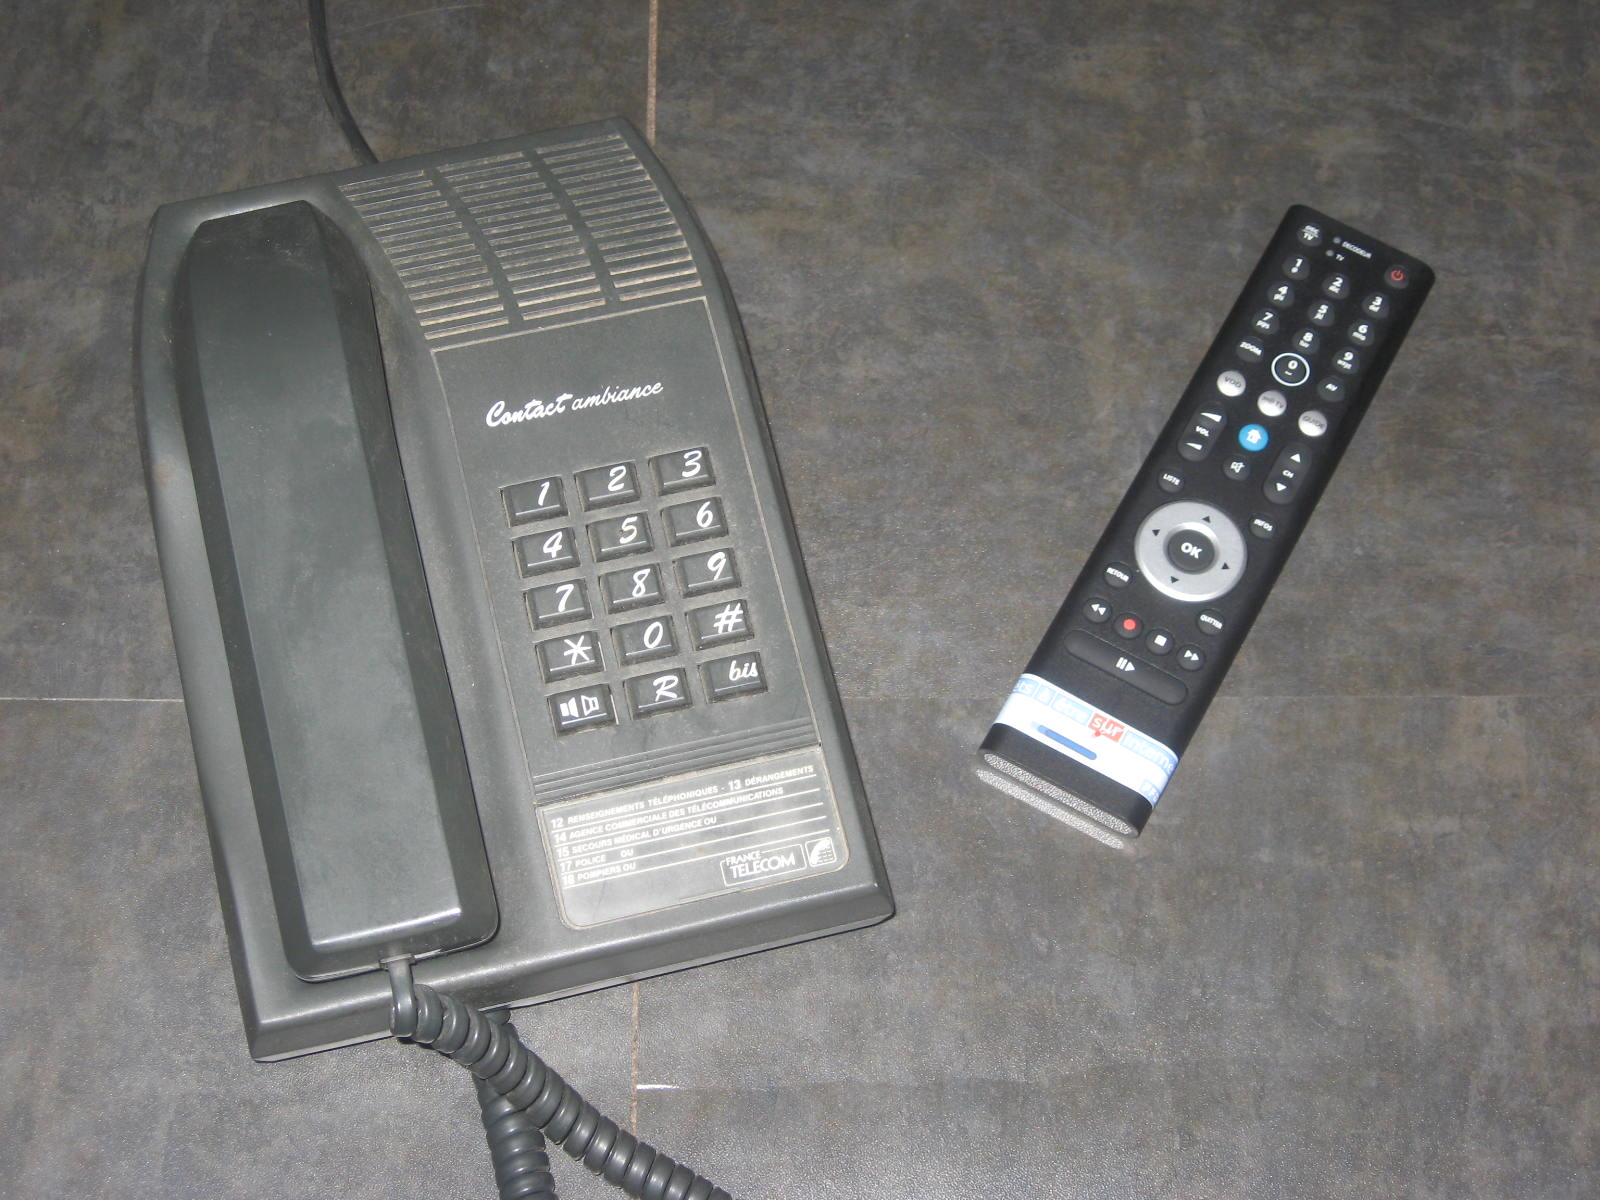
\includegraphics[width=.75\textwidth]{img2/13-photo-teltv.jpg}
\vfill
\end{center}
\end{frame}

\begin{frame}[t]
\frametitle{\textcolor{titre}{Outline}}
  \begin{center}
    The Internet Cube allow to :
    \vfill
    \begin{itemize}
      \item \textbf{Clean} easily our network access
      \item \textbf{self-host} services and personal data withouthuge computer skills
    \end{itemize}
    \end{center}
    \vfill
    \pause And it's not finish…
\end{frame}

\begin{frame}[t]{}
\begin{center}
\vfill{\Huge \textbf{Where can you find this Cube?}}
\vspace{.5cm}

{\large \emph{Because this Cube is not yet in Amazon catalog}}
\vfill
\end{center}
\end{frame}

\begin{frame}[t]
\frametitle{\textcolor{titre}{In your local associations}}
\begin{center}
\vfill
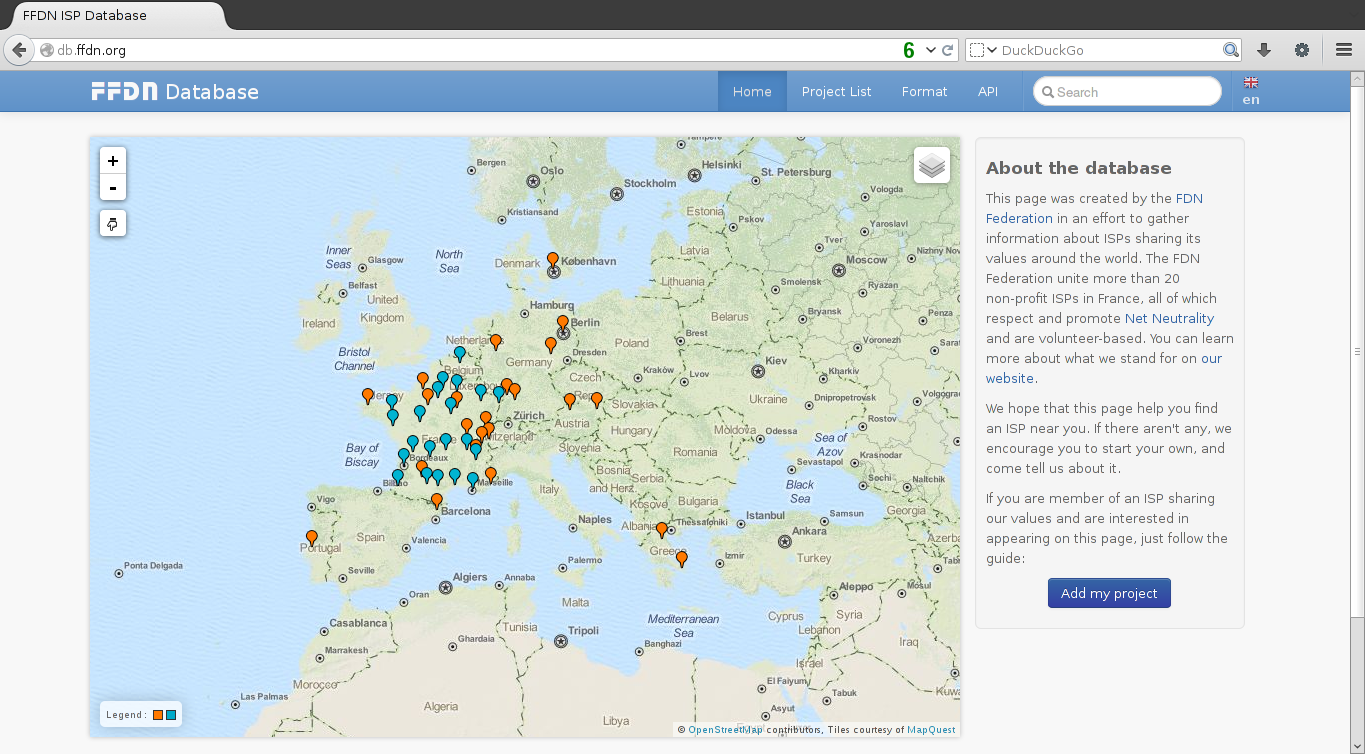
\includegraphics[width=\textwidth]{img2/25a-capture-ffdn.png}
\vfill
\end{center}
\end{frame}

\begin{frame}[t]
\frametitle{\textcolor{titre}{Or DIY because the software part is free}}
\begin{center}
\vfill
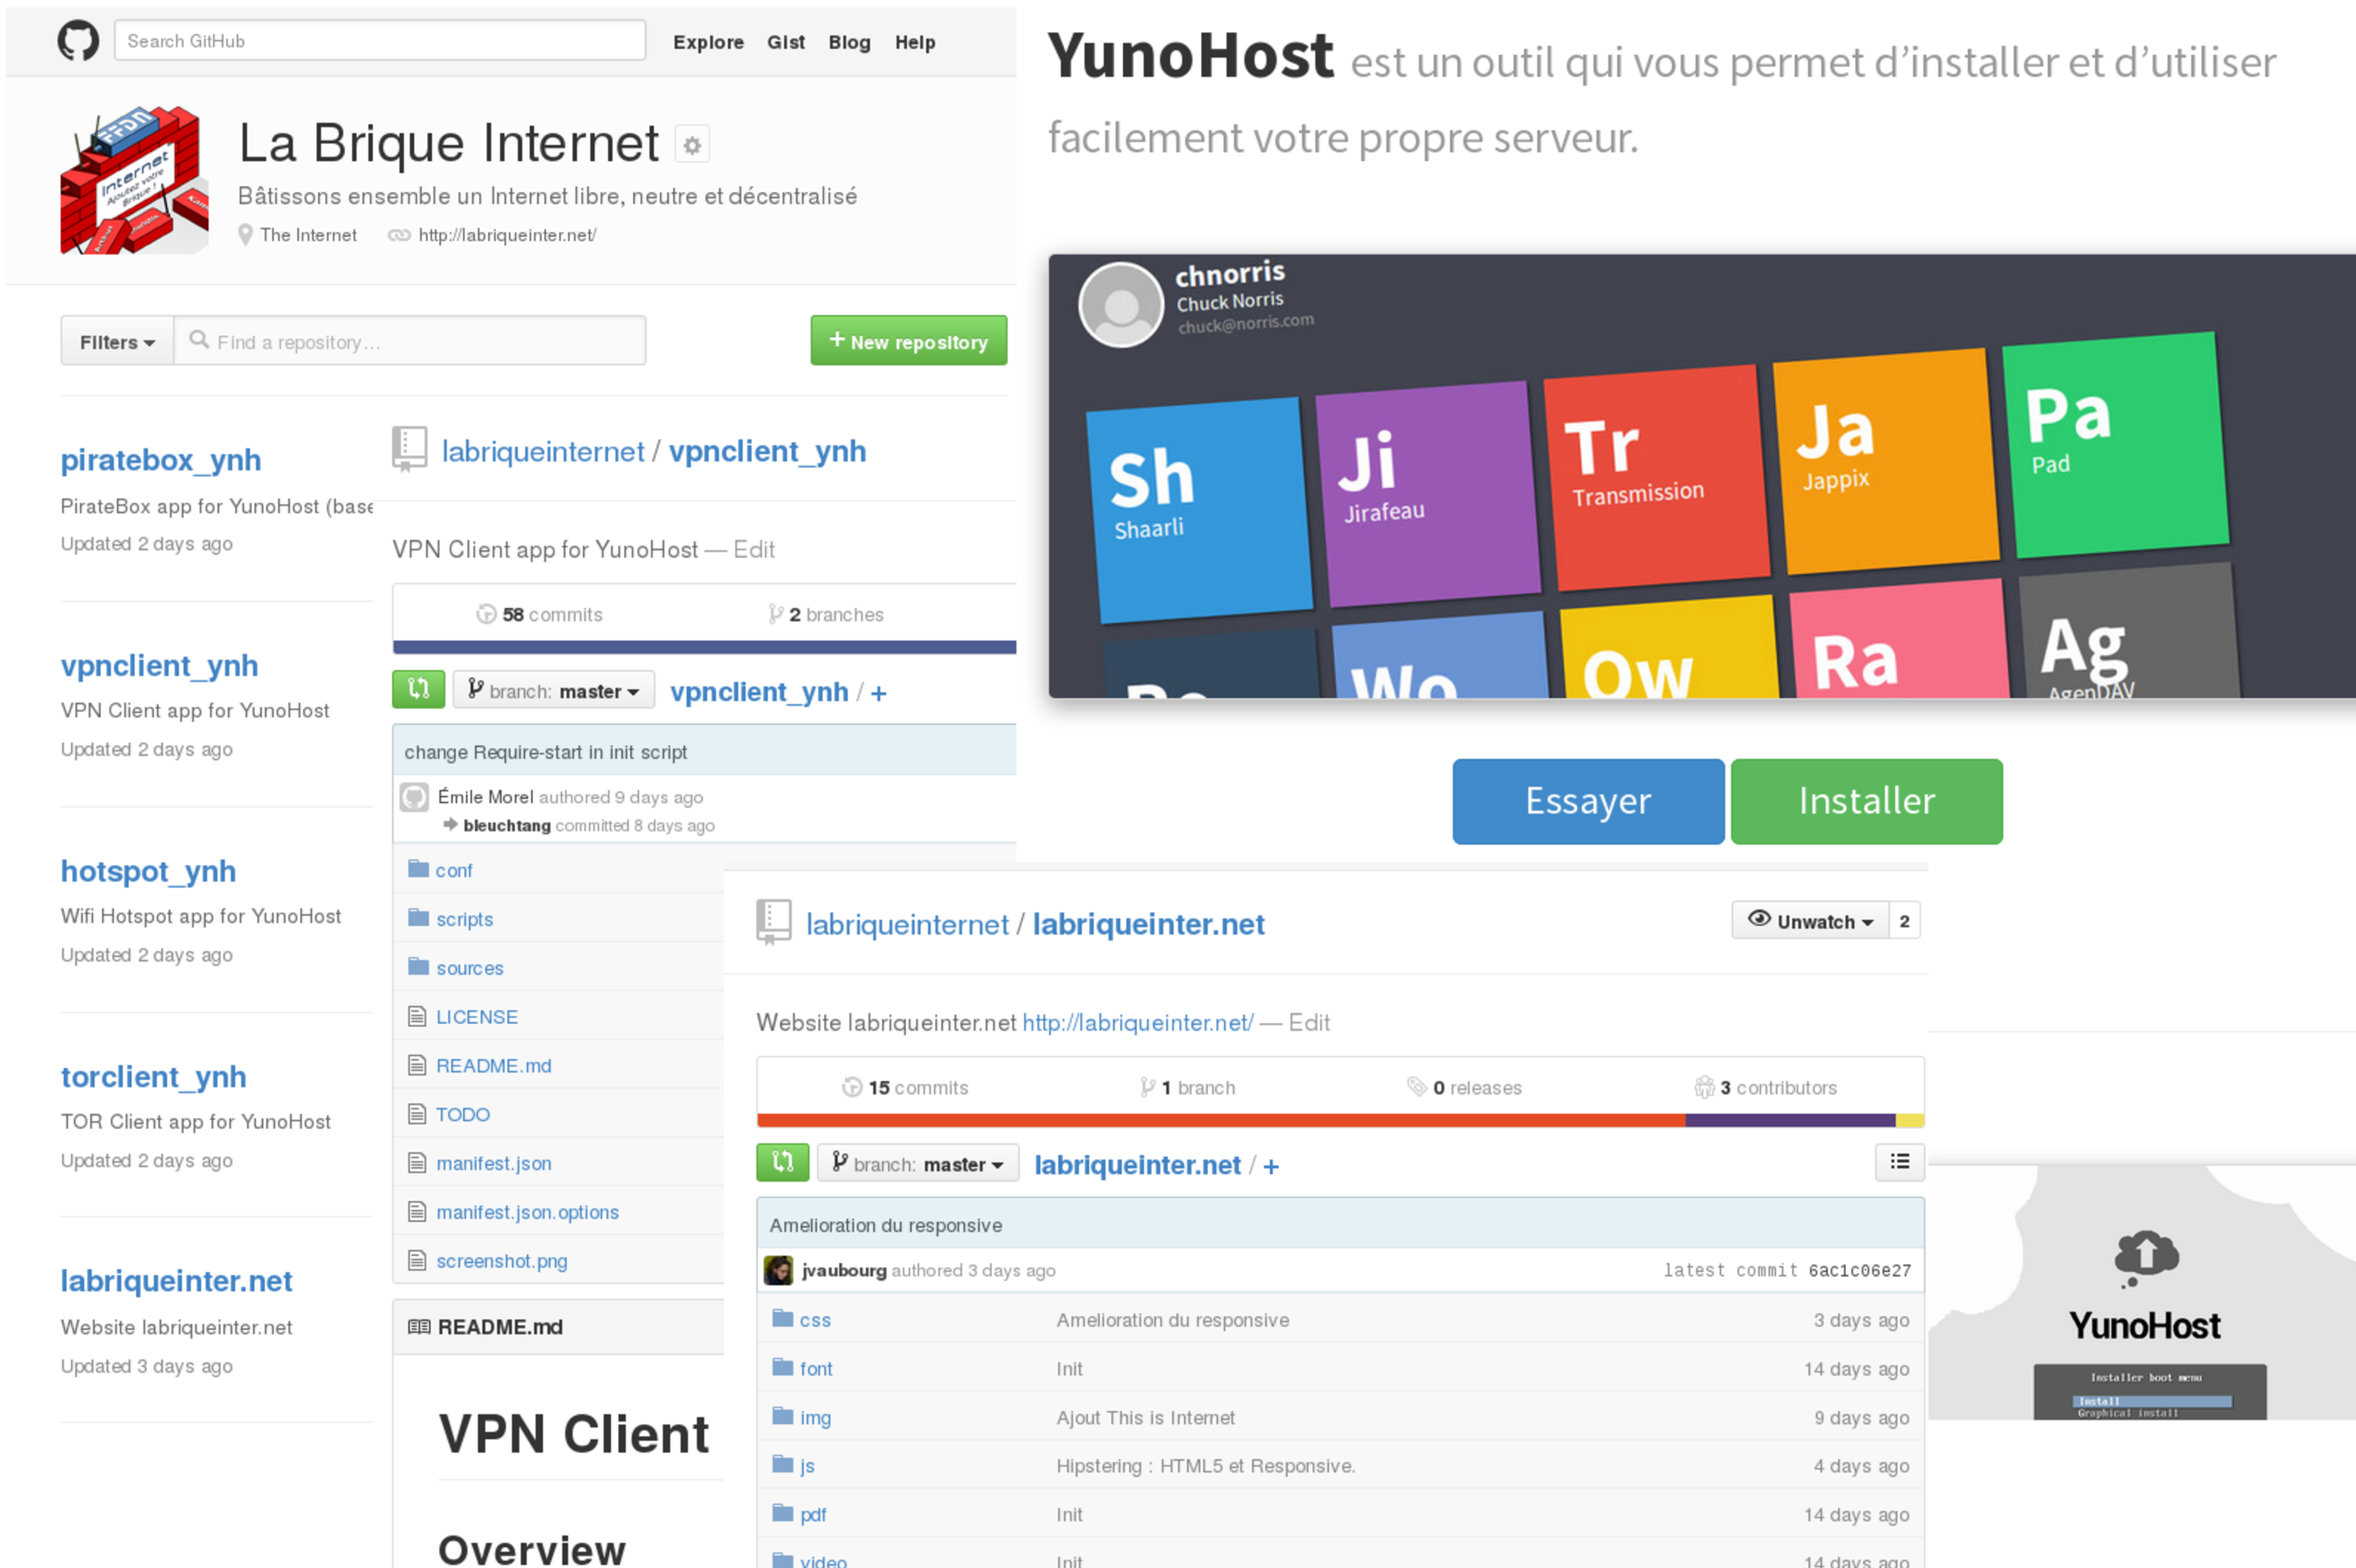
\includegraphics[width=10cm]{img2/25b-capture-github-contrib.pdf}
\vfill
\end{center}
\end{frame}

\begin{frame}[t]
\frametitle{\textcolor{titre}{And it's not finished…}}
\vfill
\begin{center}
\begin{itemize}
    \item Yunhost allows the self-hosting easily (jabber, mail, …)
    \item Just move your Cube to
    \begin{itemize}
      \item having its services, and its data with you (holidays, relocation)
      \item \textbf{to keep} its Internet access
      \item \textbf{share} with others a clean Internet access (events)
    \end{itemize}
    \pause
  \item Clean any Internet access (for example a 3G cell phone access)
  \item Have fix and public \textbf{ipv4 and ipv6} addresses
\end{itemize}
\end{center}
\end{frame}



\begin{frame}[t]
\frametitle{\textcolor{titre}{The Cube applications :}}
\vfill
\begin{center}
\begin{itemize}
    \item Neutral Internet connexion through a VPN
\end{itemize}
\end{center}
\end{frame}

\begin{frame}[t]
\frametitle{\textcolor{titre}{The VPN Cube}}
\vfill
\begin{center}
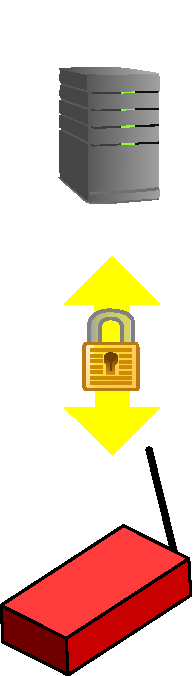
\includegraphics[scale=0.5]{img2/vpn.pdf}
\end{center}
\end{frame}

\begin{frame}[t]
\frametitle{\textcolor{titre}{The Cube applications :}}
\vfill
\begin{center}
\begin{itemize}
    \item Neutral Internet connexion through a VPN
    \item Share Box
\end{itemize}
\end{center}
\end{frame}

\begin{frame}[t]
\frametitle{\textcolor{titre}{The VPN Cube}}
\vfill
\begin{center}
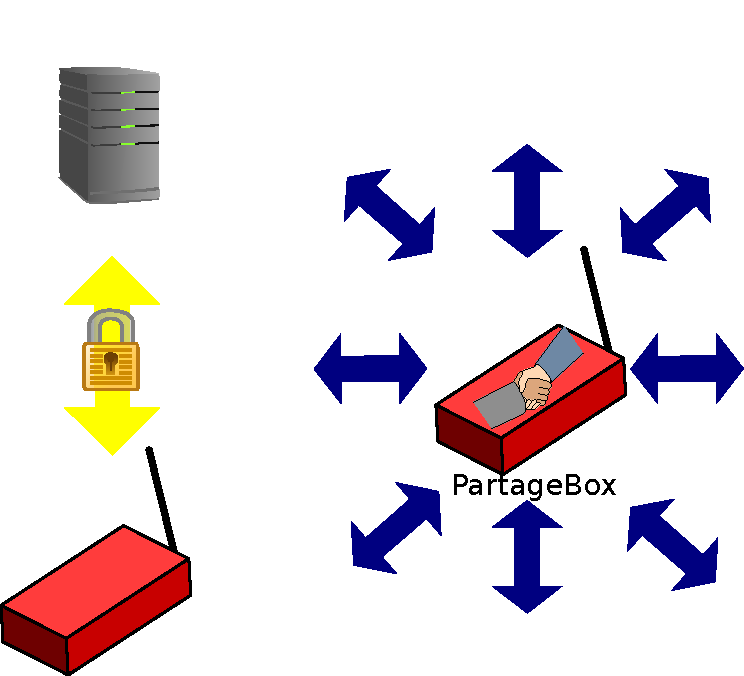
\includegraphics[scale=0.5]{img2/vpnpirate.pdf}
\end{center}
\end{frame}

\begin{frame}[t]
\frametitle{\textcolor{titre}{The Cube applications :}}
\vfill
\begin{center}
\begin{itemize}
    \item Neutral Internet connexion through a VPN
    \item Share Box
    \item Tor Access
\end{itemize}
\end{center}
\end{frame}

\begin{frame}[t]
\frametitle{\textcolor{titre}{The VPN Cube}}
\vfill
\begin{center}
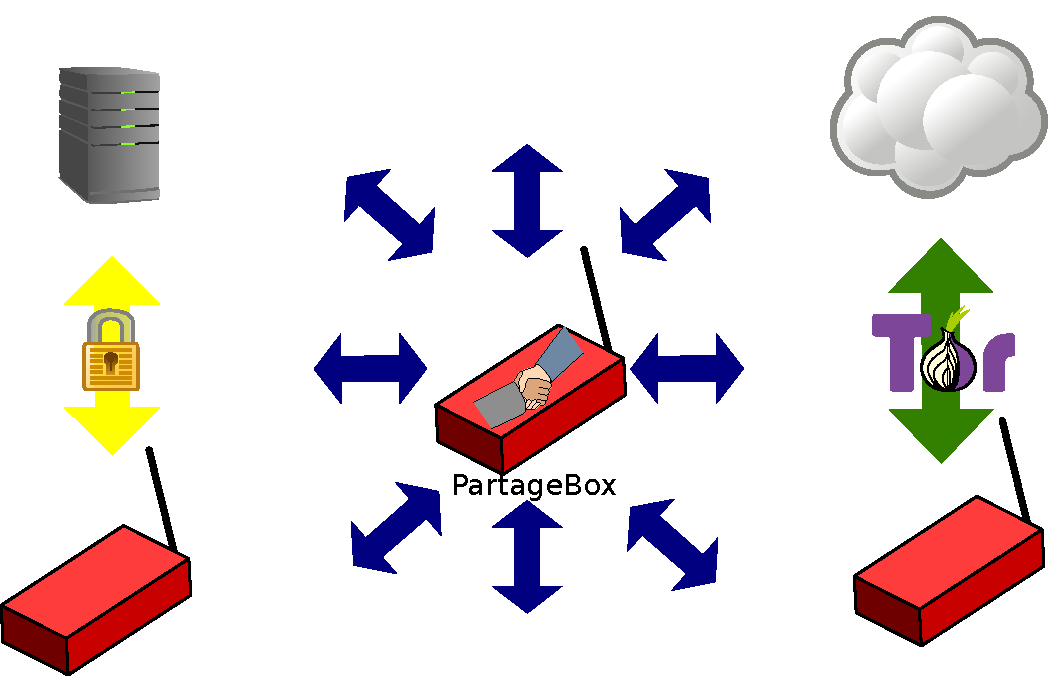
\includegraphics[scale=0.5]{img2/vpnpirator.pdf}
\end{center}
\end{frame}

\begin{frame}[t]
\frametitle{\textcolor{titre}{The Cube applications :}}
\vfill
\begin{center}
\begin{itemize}
    \item Neutral Internet connexion through a VPN
    \item Share Box
    \item Tor Access
	 \item three together (multi SSID) \good
\end{itemize}
\end{center}
\end{frame}

\begin{frame}[t]
\frametitle{\textcolor{titre}{Next step, not so far}}
\vfill
\begin{center}
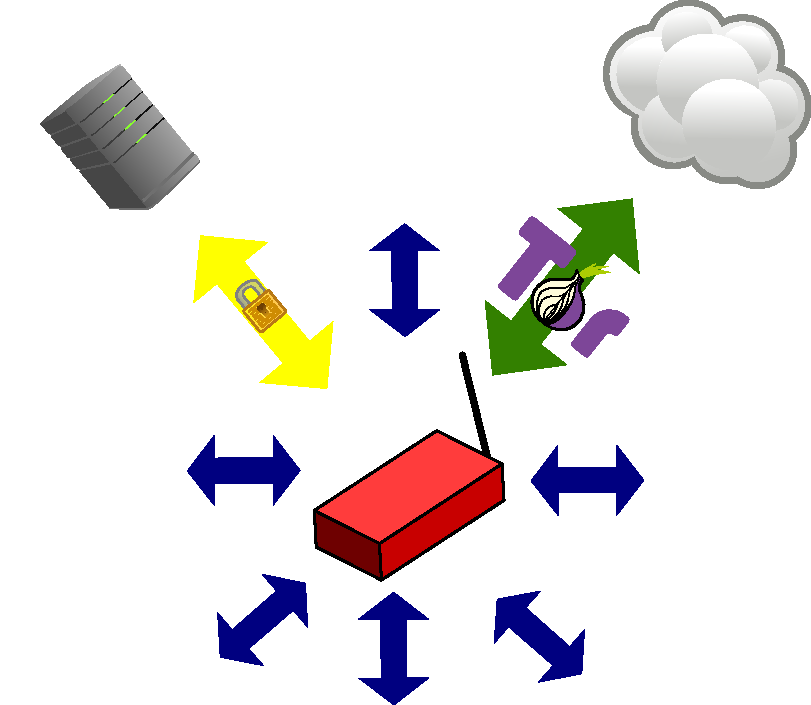
\includegraphics[scale=0.5]{img2/ultimate.pdf}
\end{center}
\end{frame}

\begin{frame}[t]
\frametitle{\textcolor{titre}{The Internet Cube, is}}
\vfill
\begin{itemize}
\item \textbf{emancipation} from the power of his ISP \vfill
\item \textbf{regain} control of its services and data \vfill
\item \textbf{use an Internet} clean peacefully
\end{itemize}
\vfill
\end{frame}

\begin{frame}[t]
\frametitle{\textcolor{titre}{The Internet Cube ?}}
\begin{center}
\vfill

\includegraphics[width=.6\textwidth]{img2/Shut-up-and-take-my-money.jpg}
\vfill
\end{center}
\end{frame}

\begin{frame}[t]
  \begin{center}
  \vfill
  \vspace{.5cm}{\Huge discussions@listes.labriqueinter.net}
  \vspace{1.5cm}
  \begin{itemize}
    \item Mailing Lists -- \url{https://listes.labriqueinter.net/}
    \item Images (beta) -- \url{https://repo.labriqueinter.net/}
    \item Build scripts -- \url{http://build.labriqueinter.net/}
  \end{itemize}
  \end{center}
\end{frame}


\begin{frame}[t]{}
\begin{center}
\vfill
\vspace{.5cm}{\Huge \url{http://LaBriqueInter.net}}
\vspace{1.5cm}
\\ To find an association near you : \vspace{.5cm} {\Large
\url{http://db.ffdn.org}}
\vfill
\end{center}
\end{frame}

\end{document}
